%%
%% This is file `mcmthesis-demo.tex',
%% generated with the docstrip utility.
%%
%% The original source files were:
%%
%% mcmthesis.dtx  (with options: `demo')
%% 
%% -----------------------------------
%% 
%% This is a generated file.
%% 
%% Copyright 
%%     2010 -- 2015 by Zhaoli Wang
%%     2014 -- 2016 by Liam Huang
%% 
%% This work may be distributed and/or modified under the
%% conditions of the LaTeX Project Public License, either version 1.3
%% of this license or (at your option) any later version.
%% The latest version of this license is in
%%   http://www.latex-project.org/lppl.txt
%% and version 1.3 or later is part of all distributions of LaTeX
%% version 2005/12/01 or later.
%% 
%% This work has the LPPL maintenance status `maintained'.
%% 
%% The Current Maintainer of this work is Liam Huang
%% 
\documentclass{mcmthesis}
\mcmsetup{CTeX = false,   % 使用 CTeX 套装时,设置为 true
        tcn = 86483, problem = E,
        sheet = true, titleinsheet = true, keywordsinsheet = true,
        titlepage = false, abstract = true}
\usepackage{palatino}
\usepackage{booktabs}
\usepackage{lipsum}
\usepackage{wrapfig}
\usepackage{geometry}
% 这两行可以让点击图片引用显示整个图片,而不是只有字
\usepackage{caption}
\captionsetup{hypcap=true}

\title{The \LaTeX{} Template for MCM Version \MCMversion}
\author{\small \href{http://www.latexstudio.net/}
  {\includegraphics[width=7cm]{mcmthesis-logo}}}
\date{\today}

\renewcommand\arraystretch{1.5}
\newcolumntype{I}{!{\vrule width 1.2pt}}
\newlength\savedwidth
\newcommand\whline{\noalign{\global\savedwidth\arrayrulewidth
                            \global\arrayrulewidth 3pt}%
                   \hline
                   \noalign{\global\arrayrulewidth\savedwidth}}
\newlength\savewidth
\newcommand\shline{\noalign{\global\savewidth\arrayrulewidth
                            \global\arrayrulewidth 1.5pt}%
                   \hline
                   \noalign{\global\arrayrulewidth\savewidth}}
% 让引用变成右上标形式,使用\upcite
\newcommand{\upcite}[1]{\textsuperscript{\textsuperscript{\cite{#1}}}}

\geometry{left=2.0cm,right=2.0cm,top=2.5cm,bottom=2.5cm}
% \geometry{top=2.5cm,bottom=2.5cm}
% 以上导言区
\begin{document}
\begin{abstract}
\lipsum[1]
\begin{keywords}
keyword1; keyword2
\end{keywords}
\end{abstract}
\maketitle
\tableofcontents
% \newpage

% \lipsum[2]
% \begin{itemize}
% \item minimizes the discomfort to the hands, or
% \item maximizes the outgoing velocity of the ball.
% \end{itemize}
% We focus exclusively on the second definition.

% \begin{itemize}
% \item the initial velocity and rotation of the ball,
% \item the initial velocity and rotation of the bat,
% \item the relative position and orientation of the bat and ball, and
% \item the force over time that the hitter hands applies on the handle.
% \end{itemize}
% \lipsum[3]
% \begin{itemize}
% \item the angular velocity of the bat,
% \item the velocity of the ball, and
% \item the position of impact along the bat.
% \end{itemize}
% \lipsum[4]
% \emph{center of percussion} [Brody 1986], \lipsum[5]

% \begin{Theorem} \label{thm:latex}
% \LaTeX
% \end{Theorem}
% \begin{Lemma} \label{thm:tex}
% \TeX .
% \end{Lemma}
% \begin{proof}
% The proof of theorem.
% \end{proof}
\newpage
\section{Introduction}
\subsection{Background}
Climate is the most important environmental condition for human activities.
Climate change has had a negative impact on the ecological environment in 
many countries and regions. It is estimated that if the coastal population 
increases and the sea level rises by 40 cm, the number of people affected by 
flood disasters will increase by 75 million to 206 million each year, 90\% of
which are in Africa and Asia. Poor people's ability to adapt to climate change 
are limited by livelihood assets and livelihood pressure. High frequency of
extreme weather events will reduce the recovery time of poverty population, 
and keep them in a fragile state for a long time. Some underdeveloped 
countries not only have to deal with the risks posed by climate change, 
but also have to deal with the impact of economic globalization, 
and are more vulnerable to failure. This phenomenon is called vulnerability.\\\\
In recent years, many international organizations have conducted vulnerability 
assessments in developing countries. The United States Agency for International
Development (USAID) famine warning system focuses on the vulnerability of 
food security in African regions. The Vulnerability Assessment committee(VAC) 
evaluated the comprehensive vulnerability of six African countries food safety 
and living condition. The Department for International Development (DFID)
focuses on rural sustainable Development and poverty alleviation in developing
countries. Vulnerability assessment is helpful for scientists and 
policymakers to understand the influence of environmental changes, 
to explore potential factors hinder the social effective response, 
to understand the vulnerable population distribution and the causes 
of vulnerability, and find out the ways to reduce vulnerability and 
increase the adaptability.
\subsection{Previous Research}
At present, many studies devote to evaluate natural ecosystem vulnerability, 
and has built many widely used quantitative methods,to figure out the 
vulnerability level and distribution of the natural ecological system, 
to predict the adaptation of natural ecosystems to risk in the future. However, 
scientists, policymakers, and ngos tend to focus more on regional 
vulnerability assessments, in order to connect with decisions. Different 
from the natural ecosystem, region is a natural-economic-social complex 
system, so the fragility of the natural ecosystem does not necessarily lead 
to a vulnerable. Human suffer from environmental impact and risk, such as 
natural disasters and limited resources, meanwhile,they adapt and transform 
the natural environment, using natural material and energy to develop itself.
Due to the complexity of the system in the region, it is difficult to 
quantitatively assess its vulnerability thus causing a gap in widely-used 
quantitative method. In the context of climate change, the situation in some
less-developed regions of the world will be severely affected, so it is 
particularly urgent to identify vulnerable areas and take measures to 
address them.


\subsection{Restatement of the Problem}
A fragile state inherently exists vulnerability of natural conditions 
like natural disasters, the decrease of the cultivated land, unpredictable 
weather and rising temperature. Coupled with the turbulent political situation, 
backward economic development, poor sanitation, the condition will get worse. 
Therefore, when considering the impact of climate on national vulnerability, 
it is not possible to consider only one single factor of climate, but also to
consider the joint role of economic, political and social factors.\\\\
However, various aspects, including climate pressure will not necessarily 
make a country vulnerable. If a country has a strong government and a high 
level of economy, the country will have a strong ability to adapt to respond
to climate change. As a result, countries are less vulnerable to climate 
change. It appears that the vulnerability of a country is not only affected
by external pressure, but more depends on the country's ability to fight 
against external pressure. In the process of modeling, we must give full 
consideration to country's ability to resist pressure and adapt.
\subsection{Our Work}
  \textbf{Work\_1, clear the definition of vulnerability and research object:} We 
  define vulnerability as the degree to which the system is susceptible to adverse effects 
  and lack of the ability to cope with adverse effects. We also define that vulnerability 
  is a function of sensitivity and adaptability. We will explain these two concepts 
  (sensitivity and adaptability) below.\\ We regard the overall vulnerability of 
  countries as a \textbf{natural-economic-social composite system} under the influence of 
  multiple factors. The vulnerability of the country is related to the country's 
  climate sensitivity index, economic development status, social stability and 
  other factors.\\\\
  \textbf{Work\_2, collect data on factors affecting national vulnerability:} The data we
  collect include sensitivity data (Extreme weather、Average precipitation in depth、Climate
  sensitivity index、Food security index、National risk index、Health index、mortality、
  Crime index、global firepower index, hunger index,  proportion of agricultural output 
  in GDP, ethnic diversity and refugee Numbers) and adaptability data(GDP per capita, 
  Poeple's Fredom index, Government Effectiveness index, Political Stability index).\\\\
  \textbf{Work\_3, calculate the correlation between climate and other factors:} we 
  calculate the relevance of various factors about economic, political, social 
  and climatic that can affect the vulnerability of the country, then choose 
  factors that are clearly relevant to climate,and \textbf{explain why and how the 
  climate affects these facts}.\\\\
  \textbf{Work\_4, build a model to measure a country's vulnerability:} Using the data 
  we collected and the data presented in the topic, we established the neural network 
  model. By taking various data(including climate factors) as the input into the model, 
  we can get the sensitivity and adaptability values. Through the function of 
  vulnerability and sensitivity and adaptability, the vulnerability value and the 
  vulnerability level can be obtained. Through our model, we can see \textbf{the direct 
  impact of vulnerability caused by climate change}. The influence of climate on other 
  factors in work\_3 shows \textbf{the indirect effect of vulnerability of the caused by 
  climate change}.\\\\
  \textbf{Work\_5, choose one country from the top ten ranking, determine how climate 
  factors affect its vulnerability:} We take data of XXX country to determine the 
  influence of climate factors on the overall vulnerability of the country.\\\\ 
  \textbf{Work\_6, choose one country apart from the top ten ranking, determine how 
  climate factors affect its vulnerability.}\\\\
  \textbf{Work\_7, Identify indicators of national vulnerability:} We grade each 
  climate factor(extreme weather, average precipitation depth, climate 
  sensitivity index). The country's vulnerability level is determined 
  by these three factors and is shown through by a list.\\\\
  \textbf{work\_8, sum up intervention measurements that can mitigate the risk of climate change.}\\\\
  \textbf{work\_9, evaluate the application scope of the model:} We select a country with large 
  territory (such as Australia) and a country with a smaller territory (e.g., 
  XXX) to evaluate the application scope of the model. And modify the model 
  to make it applicable to more general situations.
\section{Analysis of Problem}
\subsection{How to define national vulnerability?}
With the deepening of the research on vulnerability, the concept of vulnerability 
based on different subject background is also developing.\\\\
Cutter divided the vulnerability research into three categories: first, the 
vulnerability was considered as exposure; The second is to regard vulnerability 
as a social condition; The third is the combination of potential exposure 
and social elasticity.\upcite{bib18} O 'brien has a similar division, "vulnerability 
as a result" and "vulnerability as a precondition".\upcite{bib19} According to the 
description of the data given in the title, we regard the state system as a 
natural-economic-social complex system, and regard vulnerability as "the fragility 
as the result". We classify national vulnerability factors as economic, political, 
social, civic cohesion and climate change, each of which includes several detailed 
indicators. We define vulnerability as the degree to which the system is susceptible 
to adverse effects and lack of the ability to cope with adverse effects. We also 
define that vulnerability is a function of sensitivity and adaptability. 
Sensitivity is the degree to which the system is stimulated caused by multiple 
realted factors. Adaptability is the ability of a system's internal activity, 
process, structure to adapt to the external influence, and the ability to reduce 
potential losses from climate change.
\subsection{How to reflect the direct and indirect effects of climate change on national vulnerability?}
Climate change can cause direct harm to people's living environment through natural 
disasters.It can also affect agricultural production, thereby increasing 
poverty and even starvation.If combined with weak government effectiveness, 
there could be more serious consequences such as political instability and 
local wars, thus exacerbating the country's fragile state.
\section{General Assumptions and Data Analysis}
\subsection{General Assumptions}
\begin{itemize}
  \item We ignore the effects of individual factors on the model caused by year inconsistency.
  \item We assume that the overall vulnerability of the country is only determined by national sensitivity and adaptability.
  \item We assume that countries sensitivity index is determined only by extreme weather、average precipitation in depth、climate sensitivity index、food security index、national risk index、health index、mortality、arime index、global firepower index, hunger index,  proportion of agricultural output in GDP, ethnic diversity and refugee Numbers.
  \item We assume that national adaptability is determined only by GDP per capita, Poeple's Fredom index, Government Effectiveness index, Political Stability index.
  \item We assume that the factors other are independent and non-interference, but climate is not included.
  \item We assume that vulnerability can be effectively quantified by the above data.
  \item We assume that the data we collect is true and valid.
\end{itemize}
\subsection{Data Analysis}
% 表格
% \begin{table}[]
%   \centering
%   \caption{My caption}
%   \label{my-label}
%   \setlength{\tabcolsep}{7mm}{
%   \begin{tabular}{l|l|l|l|l|l|l|l|l|l|l|l}
%   \shline
%   \multicolumn{2}{lI}{\textbf{asasd}} & \multicolumn{10}{l}{\textbf{ssssssssssssssssssssss}} \\ \hline
%   \multicolumn{2}{lI}{dddd}           & \multicolumn{10}{l}{ddddddddddddddddddddd}           \\ \hline
%   \multicolumn{2}{lI}{}               & \multicolumn{10}{l}{}                                \\ \hline
%   \multicolumn{2}{lI}{}               & \multicolumn{10}{l}{}                                \\ \hline
%   \multicolumn{2}{lI}{}               & \multicolumn{10}{l}{}                                \\ \hline
%   \multicolumn{2}{lI}{}               & \multicolumn{10}{l}{}                                \\ \hline
%   \multicolumn{2}{lI}{}               & \multicolumn{10}{l}{}                                \\ \hline
%   \multicolumn{2}{lI}{}               & \multicolumn{10}{l}{}                                \\ \hline
%   \multicolumn{2}{lI}{}               & \multicolumn{10}{l}{}                                \\ \shline
%   \end{tabular}}
%   \end{table}  

\section{Variable Description and Research Method}
\subsection{Variable Description}
\subsection{Research Method}
% 插图
% \begin{figure}[h]
% \small
% \centering
% 
\includegraphics[width=12cm]{test1.jpg}
% \caption{asssssa} \label{fig:aa}
% \end{figure}

% 引用
% \eqref{aa}
% \begin{equation}
% a^2 \label{aa}
% \end{equation}

% 公式
% \[
%   \frac{\mathrm{d} C_{1}}{\mathrm{d} t}= \left 
%   ( 1-\frac{C}{R} \right )^{P_{I}}\frac{\mathrm{d} I}
%   {\mathrm{d} t}\frac{C_{I}}{I} \eqno (3)
% \]




\section{Fragile State Neural Network Model}
The study of national vulnerability indicators requires strong professional
background knowledge, but we can't derive the relationship between climate
and vulnerability through an intuitive approach from the data given in the 
problem. So, through collecting data, by using the strong self-organization, 
self-adaptive and self-learning ability of neural network, the nonlinear 
mapping of independent variables and national fragility can be completed 
without fully understanding the relationship among climate, politics, 
economy and national fragility. Combined with the above considerations, 
We established a neural network to derive a national vulnerability model 
including climatic factors.
\subsection{Model building}
\subsubsection{Introduction to the principle of BP neural network}
BP Neural Network is a kind of multi-layer feedforward neural network, 
which is mainly characterized by forward transmission and deviation back 
propagation. In forward transmission, the input signal is processed from 
the input layer through the hidden layer to the output layer. The state of 
each layer of neurons affects only the next layer of neurons. If the output 
layer does not get the desired output, it is transferred to the reverse 
propagation, and the network weight and threshold are adjusted according 
to the predicted error, so that the BP neural network prediction output 
is constantly approaching the expected output. A simple BP Neural Network 
is like Figure \ref{fig:nn} as follow.\upcite{bib20}
\begin{figure}[h]
\small
\centering
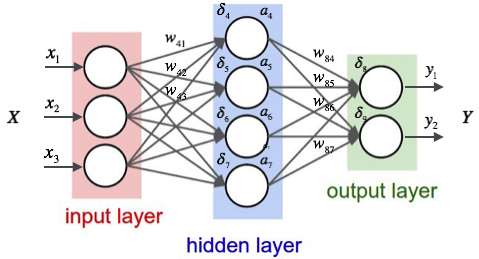
\includegraphics[width=10cm]{neuralNetwork.png}
\caption{a BP Neural Network} 
\label{fig:nn}
\end{figure}


\subsubsection{Data preprocessing}
Based on our hypothesis, the fragility of a country is related to its 
sensitivity and adaptability. Sensitivity and adaptability are closely 
related to economic conditions, political conditions, social conditions and 
climate change, and can be quantified with a numerical value. The sensitivity 
may be composed of extreme weather, the average depth of precipitation, the 
climate sensitivity index, the index of food security, the country risk index, 
the index of health, mortality, crime, global power index, hunger, agricultural 
development index, the number of ethnic diversity and refugees. Due to a variety 
of data among different indicators, some data are often hundreds of thousands of, 
and some data is within the scope of a single wave, so we each data respectively 
for the normalized processing, allow them to operations in the same numerical range, 
convenient for our model. The normalization method is as follows:
\[ y=\frac{\left ( y_{max}-y_{min} \right )\left ( x-x_{min} \right )}{x_{max}-x_{min}}+y_{min} \]
With the above formula, we can begin to build our model after the data we have 
collected is normalized. This can be done by calling the transform() function 
of sklearn.
\subsubsection{Establish BP Neural Network}
We used Google's machine learning framework, TensorFlow, to establish the BP 
neural network structure of x-n-2, where X represents the input item (that is, 
the data mentioned in the data analysis); N is the number of hidden layer neurons; 2 
represents the output item (sensitivity and adaptability). The structure diagram is 
as follows:
\begin{figure}[h]
\small
\centering
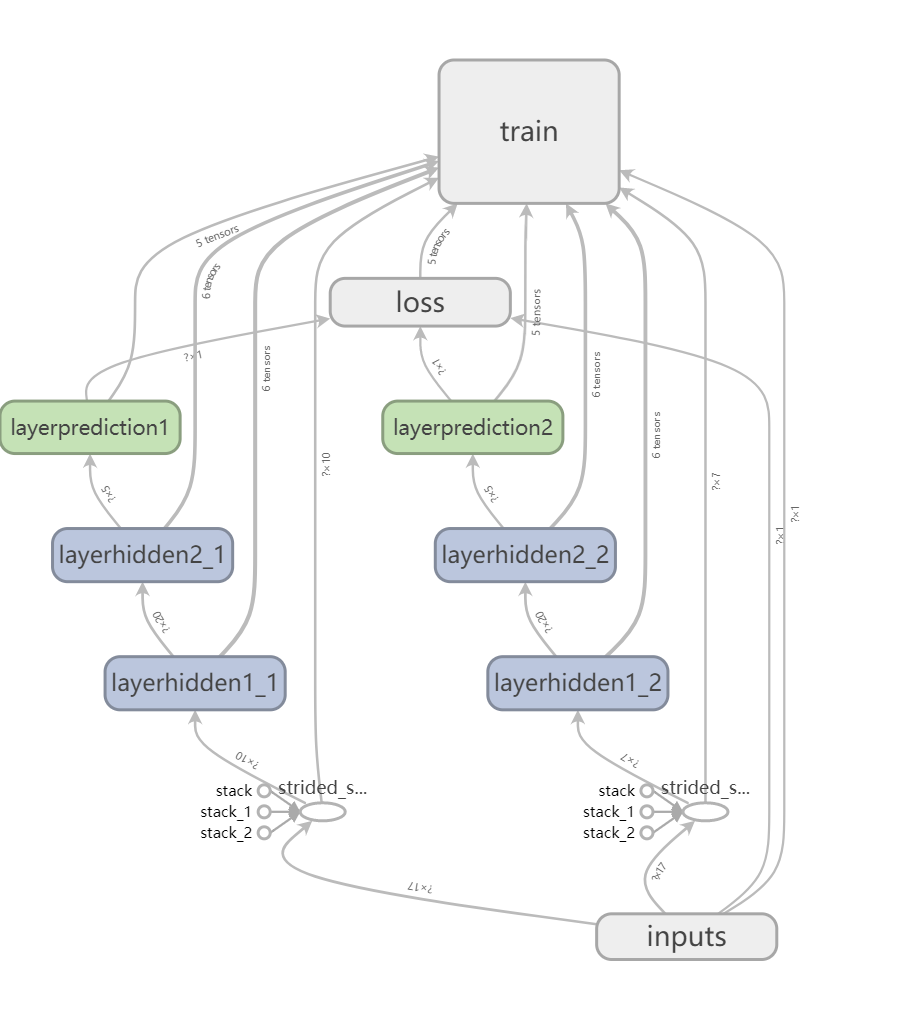
\includegraphics[width=12cm]{structure.png}
\caption{Network Structure} 
\label{fig:ns}
\end{figure}\\
We choose ReLU(Rectified Linear Unit) as hidden layer excitation function:
\[ f=max\left ( 0,w^{T}x+b \right ) \]
And linear function as the output layer Excitation function:
\[ a=n \]
The number of hidden layer neurons has a significant influence on 
the prediction accuracy of BP neural network. If the number of 
nodes is too few, the network will not learn well and the accuracy 
will be not enough. If the number of nodes is too many, the 
training time increases, the network is easy to be overfitting. 
We refer to the following formula to determine the optimal number 
of hidden layer neurons.
\[ l< n-1 \]
\[ l<\sqrt{m+n}+a \]
\[ l=\log_{2} n \]
In the formula, n is the input layer node number, L is the hidden 
layer node number, M is the output layer node number, A is the constant 
between the 0~10. In practical problems, the selection of the number 
of hidden layer nodes first uses the reference formula to determine 
the approximate range of the number of nodes, and then the optimal 
node number is determined by the method of trial-and-order. After 
many experiments, we choose n=100, at this time the BP neural network 
achieves high precision. Learning speed also has an important influence 
on the BP neural network, the learning speed is too small, the 
network learning is slow, need to increase the training times, the 
learning speed is too big, the network learns quickly, but easily 
leads to the network not to converge, affects the training precision. 
We finally decided to study at a speed of 0.01, training times 300. 
bp neural network using gradient correction method as weights and 
thresholds of learning algorithm, from the network prediction error 
in the negative gradient direction correction weights and thresholds, 
not to consider the accumulation of previous experience, learning 
process convergence is slow. For this problem, the additional momentum 
method can be used to solve the weighted value learning formula 
with additional momentum:
\[ w\left ( k \right )=
w\left ( k-1 \right )+\Delta w\left 
( k \right )+a\left [ w\left ( k-1 \right )-w\left 
( k-2 \right ) \right ] \]

\subsection{Model Testing}

\section{Sensitivity Analysis}
\subsection{Impact of x}
\subsection{Impact of y}

\section{Strengths and Weaknesses}
\subsection{Strengths of Models}
\begin{itemize}
  \item \textbf{Inclusive:} Our model contains two large indicators (sensitivity and adaptability), and 
  considers of the state's ability to intervene in natural factors such as climate. 
  Our model incorporates all aspects of the vulnerability index. The small indicators 
  in the two big indexes(sensitivity and adaptability) are composed of various political, 
  economic, climate and social sectors.
  \item \textbf{Quantification:} Our model can output a numerical value to quantify the vulnerability of a country. 
  The use of Numbers is more intuitive and more conducive to contrast, which can clearly 
  reflect changes of the vulnerability when input parameters change.
  \item \textbf{Simple but Universal:} We use the neural network model, which is relatively simple, also does not break 
  generality. If there is enough training data, each country's vulnerability index 
  can be figured out  accurate.
  \item \textbf{Visible and Understandable:} We used the plotly library of python to present the model and data 
  intuitively in the form of line graphs, which is more visualized and 
  easier to understand.
\end{itemize}


\subsection{Weaknesses of Models}
\begin{itemize}
  \item \textbf{Accuracy Relies on Statistics:} The accuracy of our model 
  depends not only on the reliability of the data itself, but also on the 
  number of training data. The more the training data has, 
  the more accurate the model is.
  \item \textbf{Not a long-term and dynamic model:} Our model is a static 
  model focusing on short-term changes. But, on the contrast, the factors 
  that affect vulnerability are long-term, dynamic and highly uncertain. 
  In terms of long-term time scale, we need to focus on future risks, and 
  we need to consider the dynamic assessment framework that changes with time. 
\end{itemize}


% 图文混排
% \begin{wrapfigure}{l}{4.5cm}%靠文字内容的左侧
%   
\includegraphics[width=4cm]{test1.jpg}\\
%   \caption{Podala Palace, Tibet}\label{fig:tibet}
%   \end{wrapfigure}

% 论文引用
\newpage
\begin{thebibliography}{99}
\bibitem{bib1} Average precipitation in depth, The World Bank, \\ 
https://data.worldbank.org/indicator/AG.LND.PRCP.MM?name\_desc=false, 
2017.
\bibitem{bib2} Droughts, floods, extreme temperatures (\% of 
population, average 1990-2009), The World Bank, 
https://data.worldbank.org/indicator/EN.CLC.MDAT.ZS, 1990-2009.
\bibitem{bib3} Global Climate Risk Index, The World Bank,\\
http://search.worldbank.org/data?qterm=climate+change\&language=\&format=,
\\viewed 7th January, 2016.
\bibitem{bib4} DEATH RATE, "The World Factbook". Cia.gov, 
\\https://www.cia.gov/library/publications/the-world-factbook/rankorder/2066rank.html,\\ 
Retrieved 2014-02-21.
\bibitem{bib5} Global Food Security Index, Food Security Index, viewed 2nd February, 2016, foodsecurityindex.eiu.com.
\bibitem{bib6} Most Dangerous Countries in the World, ATLAS \& BOOTS,\\ 
https://www.atlasandboots.com/most-dangerous-countries-in-the-world-ranked/, \\
viewed 29th January, 2017.
\bibitem{bib7} Basic Health Services by Country, www.worldmapper.org, \\
http://www.worldmapper.org/display.php?selected=220, viewed 1st August, 2016.
\bibitem{bib8} Zhang qian;Meng huixin. Social vulnerability and 
poverty under the influence of climate change: a review of foreign studies. 
Journal of agricultural university of China (social science edition), 2014, 31.2: 56-67.
\bibitem{bib9} Current World Death Rate, The World Factbook 2012,\\ 
https://www.cia.gov/library/publications/the-world-factbook/rankorder/2066rank.html, \\
viewed 27th November, 2012.
\bibitem{bib10} Refugee population by country or territory of origin, https://data.worldbank.org.
\bibitem{bib11} A. Alesina, E. La Ferrara (2005). Ethnic Diversity and Economic 
Performance. Journal of Economic Literature: 762–800. Retrieved December 15, 2016.
\bibitem{bib12} GDP per capita (current US\$),The World Bank. Accessed on 26 December 
2016, Liechtenstein updated 6. November 2016.
\bibitem{bib13} Global Hunger Index, International Food Policy Research Institute 
(IFPRI) 2011, Global Hunger Index - 2011,
http://www.ifpri.org/publication/2011-global-hunger-index, \\ 
viewed 17th October, 2011.
\bibitem{bib14} Freedom in the World 2017, freedomhouse.org,\\ 
https://freedomhouse.org/report/freedom-world/freedom-world-2017, \\ 
viewed 15th September, 2017.
\bibitem{bib15} Global FirePower Index, GFP,
http://www.globalfirepower.com/countries-listing.asp, \\ 
viewed 15th February, 2016.
\bibitem{bib16} Government Effectiveness, The Worldwide Governance 
Indicators (WGI) project, The World Bank Group, 
http://info.worldbank.org/governance/wgi/index.asp, viewed 21st October, 2011.
\bibitem{bib17} Political Stability and Absence of Violence/Terrorism, 
The Worldwide Governance Indicators (WGI) project, The World Bank Group, \\
http://info.worldbank.org/governance/wgi/index.asp, viewed 21st October, 2011.
\bibitem{bib18} Cutter S L, Boruff B J, Shirley W L. Social 
Vulnerability to Environmental Hazards. Social Science 
Quarterly, 2003, 84: 242 - 261.
\bibitem{bib19} O’Brien K, Eriksen S, Schjolen A, et al. What’s in a Word?, 
Conflicting Interpretations of Vulnerability in Climate Change Research. CICERO Working Paper, 2004(4)
\bibitem{bib20} matlab neural network 30 case analysis, Matlab Chinese BBS, Beijing: Beijing aerospace university press, 2010.
\end{thebibliography}

% 附录
\begin{appendices}

\section{First appendix}

\lipsum[13]

Here are simulation programmes we used in our model as follow.\\

\textbf{\textcolor[rgb]{0.98,0.00,0.00}{Input matlab source:}}
\lstinputlisting[language=Matlab]{./code/mcmthesis-matlab1.m}

\section{Second appendix}

some more text \textcolor[rgb]{0.98,0.00,0.00}{\textbf{Input C++ source:}}
\lstinputlisting[language=C++]{./code/mcmthesis-sudoku.cpp}

\end{appendices}
\end{document}

%% 
%% This work consists of these files mcmthesis.dtx,
%%                                   figures/ and
%%                                   code/,
%% and the derived files             mcmthesis.cls,
%%                                   mcmthesis-demo.tex,
%%                                   README,
%%                                   LICENSE,
%%                                   mcmthesis.pdf and
%%                                   mcmthesis-demo.pdf.
%%
%% End of file `mcmthesis-demo.tex'.
